\begin{frame}{Self-Consistency}
  \begin{itemize}
    \item \textbf{Self-Consistency} aims to improve on the naive greedy decoding used in chain-of-thought prompting
    \item The idea is to sample multiple, diverse \textbf{reasoning paths} through few-shot CoT, and use the generations to select the most \textbf{consistent answer}.
    \item This helps to boost the performance of CoT prompting on tasks involving arithmetic and \textbf{commonsense reasoning}
  \end{itemize}

  \begin{center}
    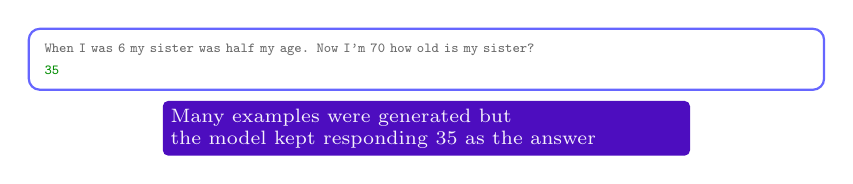
\begin{tikzpicture}
      % Code box for the prompt and answer
      \node[
        draw=blue!60,
        thick,
        rounded corners=4pt,
        fill=white,
        anchor=north west,
        inner sep=2mm,
        font=\ttfamily\tiny,
        text width=9.7cm,
        align=left,
        text=gray!82!black
      ] (codebox) at (0,0) {%
When I was 6 my sister was half my age. Now I'm 70 how old is my sister?\\[0.3em]
\textcolor{green!55!black}{35}
      };

      % Annotation box below with purple background
      \node[
        draw=none,
        fill=purple!35!blue,
        fill opacity=0.95,
        rounded corners=2pt,
        inner sep=2.8pt,
        font=\scriptsize,
        text=white,
        text width=6.5cm,
        align=left,
        anchor=north,
      ] (annbox) at ([yshift=-1.2mm]codebox.south) {%
Many examples were generated but\\the model kept responding 35 as the answer
      };
 
    \end{tikzpicture}
  \end{center}

  \vspace{0.2em}
  {\scriptsize
    \color{gray!75!black}
    Source: \url{https://arxiv.org/abs/2201.11903} (adapted presentation, Lady Margaret Hall, Oxford)
  }
\end{frame}

\begin{frame}[fragile]{Self-Consistency Example}
  \begin{center}
    \begin{tikzpicture}
      % Main Prompted Reasoning Paths Example Box (blue border)
      \node[
        draw=blue!60,
        thick,
        rounded corners=4pt,
        fill=white,
        anchor=north west,
        inner sep=2.6mm,
        font=\ttfamily\tiny,
        text width=8.8cm,
        align=left,
        text=gray!88!black
      ] (mainbox) at (0,0) {%
\textbf{Q:} There are 25 trees in the grove. Grove workers will plant trees in the grove today. When they are done, there will be 34 trees. How many trees did the grove workers plant today?\\
\textbf{A:} 34 - 25 = \textcolor{orange!80!black}{9}.\\[0.5em]
\textbf{Q:} At school, Livia has 12 tulips. Her friend Liana has 8 tulips. The difference must be the number of extra they planted. So, they must have planted 12 - 8 = \textcolor{orange!80!black}{4}.\\[0.4em]
\textbf{Q:} If there are 3 cars in the parking lot and 2 more cars arrive, how many cars are now in parking lot?\\
There were 3 cars and 2 arrived, so 3 + 2 = \textcolor{orange!80!black}{5}.\\[0.4em]
\textbf{Q:} Olivia has \$23. She bought five bagels for \$3 each. How much money does she have left?\\
She bought 5 bagels for \$3 each. This means she spent 5 $\times$ 3 = \$15. So, 23 - 15 = \textcolor{orange!80!black}{8}.\\[0.4em]
\textbf{Q:} When I was 6 my sister was half my age. Now I'm 70, how old is my sister?%
      };
 

      % First sampled output (green highlight)
      \node[
        draw=black!30,
        fill=green!24!white,
        rounded corners=2pt,
        inner sep=3pt,
        font=\scriptsize\ttfamily,
        text width=9.8cm,
        align=left,
        text=black,
        anchor=north west
      ] (a1) at ([yshift=-1.20em]mainbox.south west) {%
\texttt{When I was 6 my sister was half my age. She was 3. Now I'm 70, so she must be 3 years younger, which is 67.}
      };

      % Second sampled output
      \node[
        draw=black!20,
        fill=green!17!white,
        rounded corners=2pt,
        inner sep=3pt,
        font=\scriptsize\ttfamily,
        text width=9.8cm,
        align=left,
        text=black,
        anchor=north west
      ] (a2) at ([yshift=-0.25em]a1.south west) {%
\texttt{When the narrator was 6, his sister was half his age, which is 3. Now, the narrator is 70, his sister would be 3 years younger: 67.}
      };

      % Third sampled output
      \node[
        draw=black!14,
        fill=green!10!white,
        rounded corners=2pt,
        inner sep=3pt,
        font=\scriptsize\ttfamily,
        text width=9.8cm,
        align=left,
        text=black,
        anchor=north west
      ] (a3) at ([yshift=-0.25em]a2.south west) {%
\texttt{When the narrator was 6, his sister was half his age, which is 3. Now that the narrator is 70, his sister would be 3 years younger, so 70 - 3 = 67 years old.}
      };

      % Vertical "Sampled Outputs" label (rotated)
      \node[
        font=\scriptsize\bfseries,
        text=gray!70!black,
        anchor=south,
        align=center,
        rotate=90
      ] at ([xshift=-0.78cm,yshift=-2.3em]mainbox.south west) {Sampled\\Outputs};

      % Draw a blue border around mainbox and all answer boxes for clarity
      \draw[draw=blue!60, thick, rounded corners=4pt]
        ([xshift=-0.12cm,yshift=0.20cm]mainbox.north west) rectangle ([xshift=0.13cm,yshift=-0.24cm]a3.south east);

      % KAUST & LMH logo box (approximated, top right)
      \node[
        anchor=north east,
        inner sep=2pt
      ] at ([xshift=0.04cm]mainbox.north east)
      {\includegraphics[height=0.7cm]{kaust-logo-placeholder}\hspace{0.6em}\includegraphics[height=0.7cm]{lmh-logo-placeholder}};

    \end{tikzpicture}
  \end{center}
\end{frame}
